\documentclass[tikz]{standalone}
\usepackage{fontspec}
\renewcommand*{\familydefault}{\sfdefault}
\usepackage{standalone}
\usepackage{amssymb}
\usetikzlibrary{decorations}
%\usetikzlibrary{arrows.meta, decorations.pathmorphing, decorations.pathreplacing, shapes.geometric}
\usetikzlibrary{bayesnet}

\begin{document}
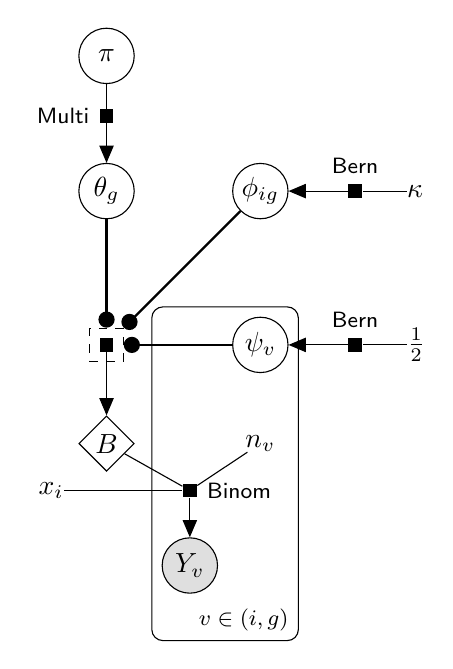
\begin{tikzpicture}%[font=\footnotesize, xscale=1.5]

\node[det]                    (B)   {$B$}; %
\factor[above=0.8 of B]       {B-f} {} {} {}; %
\draw[->] (B-f) -- (B);

% theta_iv
\node[latent, above=1.5 of B-f] (theta) {\(\theta_g\)};
\gate {} {(B-f)} {theta} ; %

% psi_v
\node[latent, right=1.5 of B-f] (psi) {\(\psi_v\)};
\gate {} {(B-f)} {psi} ; %
\node[const, right=1.5 of psi] (half) {\(\frac{1}{2}\)};
\factor[right=0.75 of psi, label=Bern]       {psi-f} {} {} {}; %
\factoredge {half} {psi-f} {psi};

% phi_ig
\node[latent] (phi) at (theta -| psi) {\(\phi_{ig}\)} ;
\gate {} {(B-f)} {phi} ; %
\factor[right=0.75 of phi, label=Bern]       {phi-f} {} {} {}; %
\node[const, right=1.5 of phi] (kappa) {\(\kappa\)} ;
\factoredge {kappa} {phi-f} {phi};

% Y_v
\node[const] (n) at (B -| psi) {\(n_v\)};
\path (B) -- (n) coordinate[midway] (B-n);
\node[factor, below=0.5 of B-n] (Y-f) [label=right:Binom] {};
\node[obs, below=0.5 of Y-f] (Y) {\(Y_v\)};
\node[const, left=1.5 of Y-f] (x) {\(x_i\)};

\factoredge {B,n,x} {Y-f} {Y};

\plate {} {(Y) (n) (psi)} {\(v\in(i,g)\)};

\factor[above=0.5 of theta, label=left:Multi]       {theta-f} {} {} {}; %
\node[latent, above=1.0 of theta] (pi) {\(\pi\)};
\factoredge {pi} {theta-f} {theta};
\end{tikzpicture}
\end{document}
